\documentclass{article}

\usepackage{fancyhdr}
\usepackage{extramarks}
\usepackage{amsmath,mathrsfs,amssymb}
\usepackage{amsthm}
\usepackage{amsfonts}
\usepackage{tikz}
\usepackage[plain]{algorithm}
\usepackage{algpseudocode}
\usepackage[]{mcode}
\usepackage{graphicx}
\usepackage{pgfplots}
\usepackage{xfrac}
\usepackage{caption}
\usepackage{epstopdf}
\usepackage{siunitx}

\usetikzlibrary{automata,positioning}

%
% Basic Document Settings
%

\topmargin=-0.45in
\evensidemargin=0in
\oddsidemargin=0in
\textwidth=6.5in
\textheight=9.0in
\headsep=0.25in

\linespread{1.1}

\pagestyle{fancy}
\lhead{\hmwkAuthorName}
\chead{\hmwkClass\ (\hmwkClassInstructor\ \hmwkClassTime): \hmwkTitle}
\rhead{\firstxmark}
\lfoot{\lastxmark}
\cfoot{\thepage}

\renewcommand\headrulewidth{0.4pt}
\renewcommand\footrulewidth{0.4pt}

\setlength\parindent{0pt}

%
% Create Problem Sections
%

\newcommand{\enterProblemHeader}[1]{
    \nobreak\extramarks{}{Problem \arabic{#1} continued on next page\ldots}\nobreak{}
    \nobreak\extramarks{Problem \arabic{#1} (continued)}{Problem \arabic{#1} continued on next page\ldots}\nobreak{}
}

\newcommand{\exitProblemHeader}[1]{
    \nobreak\extramarks{Problem \arabic{#1} (continued)}{Problem \arabic{#1} continued on next page\ldots}\nobreak{}
    \stepcounter{#1}
    \nobreak\extramarks{Problem \arabic{#1}}{}\nobreak{}
}

\setcounter{secnumdepth}{0}
\newcounter{partCounter}
\newcounter{homeworkProblemCounter}
\setcounter{homeworkProblemCounter}{1}
\nobreak\extramarks{Problem \arabic{homeworkProblemCounter}}{}\nobreak{}

%
% Homework Problem Environment
%
% This environment takes an optional argument. When given, it will adjust the
% problem counter. This is useful for when the problems given for your
% assignment aren't sequential. See the last 3 problems of this template for an
% example.
%
\newenvironment{homeworkProblem}[1][-1]{
    \ifnum#1>0
        \setcounter{homeworkProblemCounter}{#1}
    \fi
    \section{Problem \arabic{homeworkProblemCounter}}
    \setcounter{partCounter}{1}
    \enterProblemHeader{homeworkProblemCounter}
}{
    \exitProblemHeader{homeworkProblemCounter}
}

%
% Homework Details
%   - Title
%   - Due date
%   - Class
%   - Section/Time
%   - Instructor
%   - Author
%

\newcommand{\hmwkTitle}{Tutorial\ 3}
\newcommand{\hmwkDueDate}{April 25, 2016}
\newcommand{\hmwkClass}{Systems Modelling and Control}
\newcommand{\hmwkClassTime}{}
\newcommand{\hmwkClassInstructor}{Damien Hill}
\newcommand{\hmwkAuthorName}{S.Reynolds (262538)}

%
% Title Page
%

\title{
    \vspace{2in}
    \textmd{\textbf{\hmwkClass:\ \hmwkTitle}}\\
    \normalsize\vspace{0.1in}\small{Due\ on\ \hmwkDueDate\ at 3:10pm}\\
    \vspace{0.1in}\large{\textit{\hmwkClassInstructor\ \hmwkClassTime}}
    \vspace{3in}
}

\author{\textbf{\hmwkAuthorName}}
\date{}

\renewcommand{\part}[1]{\textbf{\large Part \Alph{partCounter}}\stepcounter{partCounter}\\}

%
% Various Helper Commands
%

% Useful for algorithms
\newcommand{\alg}[1]{\textsc{\bfseries \footnotesize #1}}

% For derivatives
\newcommand{\deriv}[1]{\frac{\mathrm{d}}{\mathrm{d}x} (#1)}

% For partial derivatives
\newcommand{\pderiv}[2]{\frac{\partial}{\partial #1} (#2)}

% Integral dx
\newcommand{\dx}{\mathrm{d}x}

% Alias for the Solution section header
\newcommand{\solution}{\textbf{\large Solution}}

% Probability commands: Expectation, Variance, Covariance, Bias
\newcommand{\E}{\mathrm{E}}
\newcommand{\Var}{\mathrm{Var}}
\newcommand{\Cov}{\mathrm{Cov}}
\newcommand{\Bias}{\mathrm{Bias}}

\DeclareMathOperator{\sinc}{sinc}

\graphicspath{{./fig/}}

\begin{document}

\maketitle

\pagebreak

%%%%%%%%%%%%%%%%%%%%%%%%%%%%%%%%%%%%%%%%%%%%%%%%%%%%%%%%%%%%%%%%%%%%%%%%%%%%%%%%%%%%%%%%%%%%%%%%%%%%%%%%%%%%%%%%%%%%%%
% Question 1
%%%%%%%%%%%%%%%%%%%%%%%%%%%%%%%%%%%%%%%%%%%%%%%%%%%%%%%%%%%%%%%%%%%%%%%%%%%%%%%%%%%%%%%%%%%%%%%%%%%%%%%%%%%%%%%%%%%%%% 

\begin{homeworkProblem}
    
    
    \textbf{Frequency Response}\\
    
    \textsc{Question a}\\
    
    A linear time-invariant continuous-time system has some frequency function $H(\omega)$. Some input $x(t)$, which is composed of a DC component and 2 sinusoids with distinct multiples of some fundamental frequency, $w_0$, is given as:
    \begin{align*}
	    x(t)	&= 1 + 4\cos(2 \pi t) + 8\sin(3 \pi t - \sfrac{\pi}{2})\\
				&= 1 + 4\cos(2 \pi t) + 8\cos(3 \pi t - \pi)
    \end{align*}
    
    The fundamental frequency of the sinusoids, $w_0$, is the lowest common divisor of $2 \pi$ and $3 \pi$. Hence, the fundamental frequency is given by:
    
    \begin{align*}
	    w_0 = \pi
    \end{align*}
    
    The output to the system, $y(t)$, is given by:
    
    \begin{align*}
	    y(t)	&= 2 - 2\sin(2 \pi t)\\
			    &= 2 + 2\sin(- 2 \pi t)\\
			    &= 2 + 2\cos(- 2 \pi t - \sfrac{\pi}{2})\\
			    &= 2 + 2\cos\big(-(2 \pi + \sfrac{\pi}{2})\big)\\
				&= 2 + 2\cos(2 \pi t + \sfrac{\pi}{2})
    \end{align*}
    
    Now, the above input signal, $x(t)$, is periodic and as such has the complex Fourier series representation:
    
    \begin{align*}
	    x(t) = \sum_{k = -\infty}^{\infty} c^{x}_k e^{jk \omega_0 t}
    \end{align*}
    
    A single instance, $k$, of this infinite series is given by:
    
    \begin{align*}
	    x_k(t) = c^{x}_k e^{jk \omega_0 t}
    \end{align*}
    
	Because the system is linear, we can apply the transfer function to each instance of complex Fourier series representation of $x(t)$, and rely on superposition to obtain the output, $y(t)$. This is represented as:
	
	\begin{align*}
		y(t) = \sum_{k = -\infty}^{\infty} H(\omega_0 k) c^{x}_{k} e^{jk \omega_0 t}
	\end{align*} 
    
    A single instance, $k$, of the infinite Fourier series representing $y(t)$ can be written as:
    
    \begin{align*}
	    y_{k}(t) = c^{y}_{k}e^{jk \omega_0 t} = H(\omega_0 k) c^{x}_{k} e^{jk \omega_0 t}
    \end{align*}
    
    \newpage
    
    Hence, we can see that:
    
    \begin{align*}
	    c^{y}_{k} = H(\omega_0 k) c^{x}_{k}
    \end{align*}
    
    Which allows us to write an expression for the transfer function, $H(\omega)$, in terms of $c^{x}_{k}$ and $c^{y}_{k}$:
    
    \begin{align*}
	    H(\omega) = H(k \omega_0) = \frac{c^{y}_{k}}{c^{x}_{k}}, \quad \omega = k \omega_0
    \end{align*}
    
    Hence, $\exists$ $H(\omega)$  $\forall$ $c^{x}_{k} \neq 0$. That is to say, we can find $H(\omega)$ for $k = 0, 2, 3$.\\
    
    \vspace{5mm}
    
    \textsc{Question 2}\\
    
    $H(\omega) = H(k \omega_0)$ can be found for $k = 0, 2, 3$. We first note that:
    
    \begin{align*}
	    c^{x}_{0} 	&= 1\\
	    c^{x}_{2} 	&= \frac{1}{2} \cdot 4 = 2\\
	    c^{x}_{3} 	&= \frac{1}{2} \cdot 8 \cdot e^{-j \pi} = 4 \cdot e^{-j \pi}
    \end{align*}
    
    Further, we can see that:
    
    \begin{align*}
	    c^{y}_{0} &= 2\\
	    c^{y}_{2} &= \frac{1}{2} \cdot 2 \cdot e^{j \cdot \sfrac{\pi}{2} } = e^{j \cdot \sfrac{\pi}{2} }\\
	    c^{y}_{3} &= 0
    \end{align*}
    
    Hence, we get that:
    
    \begin{align*}
	    H(0 \cdot \pi) &= \frac{c^{y}_{0}}{c^{x}_{0}} = \frac{2}{1} = 2\\
	    H(2 \cdot \pi) &= \frac{c^{y}_{2}}{c^{x}_{2}} = \frac{e^{j \cdot \sfrac{\pi}{2} }}{2} = \frac{1}{2} \cdot e^{j \cdot \sfrac{\pi}{2} }\\
	    H(3 \cdot \pi) &= \frac{c^{y}_{3}}{c^{x}_{3}} = \frac{0}{4 \cdot e^{-j \pi}} = 0
    \end{align*} 
    
\end{homeworkProblem}

\newpage

%%%%%%%%%%%%%%%%%%%%%%%%%%%%%%%%%%%%%%%%%%%%%%%%%%%%%%%%%%%%%%%%%%%%%%%%%%%%%%%%%%%%%%%%%%%%%%%%%%%%%%%%%%%%%%%%%%%%%%
% Question 2
%%%%%%%%%%%%%%%%%%%%%%%%%%%%%%%%%%%%%%%%%%%%%%%%%%%%%%%%%%%%%%%%%%%%%%%%%%%%%%%%%%%%%%%%%%%%%%%%%%%%%%%%%%%%%%%%%%%%%%

\begin{homeworkProblem}
    
    \textbf{Filtering of sound}\\
    
    Suppose a continuous-time signal, $x(t)$, is given by the following:
    
    \begin{align*}
	    x(t) = \cos(440 \cdot 2 \pi \cdot t) + \cos(554 \cdot 2 \pi \cdot t) + \cos(659 \cdot 2 \pi \cdot t)
    \end{align*}
	
	To play the sound of this signal for 2 seconds, the following Matlab code was implemented:
	
	\begin{lstlisting}
		% Script plays audio of signal x(t)
		dur = 2.0;
		fs = 44100;
		t = 0:(1/fs):dur;
	
		% Complex representation of the signal
		xe1 = 0.5*(exp(1i*440*2*pi*t) + exp(-1i*440*2*pi*t));
		xe2 = 0.5*(exp(1i*554*2*pi*t) + exp(-1i*554*2*pi*t));
		xe3 = 0.5*(exp(1i*659*2*pi*t) + exp(-1i*659*2*pi*t));
	
		x = xe1 + xe2 + xe3;
	
		sound(x,fs)
	\end{lstlisting}
	
\end{homeworkProblem}



%%%%%%%%%%%%%%%%%%%%%%%%%%%%%%%%%%%%%%%%%%%%%%%%%%%%%%%%%%%%%%%%%%%%%%%%%%%%%%%%%%%%%%%%%%%%%%%%%%%%%%%%%%%%%%%%%%%%%%
% Question 3
%%%%%%%%%%%%%%%%%%%%%%%%%%%%%%%%%%%%%%%%%%%%%%%%%%%%%%%%%%%%%%%%%%%%%%%%%%%%%%%%%%%%%%%%%%%%%%%%%%%%%%%%%%%%%%%%%%%%%%

\begin{homeworkProblem}
    
    \textbf{Filtering of sound}\\
    
    Suppose a continuous-time signal, $x(t)$, is given by the following:
    \begin{align*}
    x(t) = \cos(440 \cdot 2 \pi \cdot t) + \cos(554 \cdot 2 \pi \cdot t) + \cos(659 \cdot 2 \pi \cdot t)
    \end{align*}
    
    The representation of a periodic signal as a complex Fourier series can be written as follows:
    \begin{align*}
	    x(t) = \sum_{k = -\infty}^{\infty} c^{x}_{k} e^{jk \omega_0 t}
    \end{align*}
    
    The complex coefficients, $c^{x}_{k}$, can be written as:
    \begin{align*}
	    c^{x}_{k} = \frac{1}{2} \cdot A_k \cdot e^{j \theta_k}
    \end{align*}
    
    It must be noted that $|c^{x}_{k}| = |c^{x}_{-k}| = \frac{A_k}{2}$ $\forall$ $k \in \mathbb{Z^+}$, however, the same is not true for $\angle c^{x}_{k}$. In fact, $\angle c^{x}_{k} = -\angle c^{x}_{-k}$ $\forall$ $k \in \mathbb{Z^+}$.\\
    
    For the signal in this problem we note that $w_0 = 2 \pi$, which greatly simplifies the complex Fourier series representation since there are only three terms in the sequence whose amplitudes are non-zero: $k = 440$, $k = 554$,and $k = 659$. Further, we see that $A_{440} = A_{554} = A_{659} = 1$, and that $\theta_{440} = \theta_{554} = \theta_{659} = 0$. Hence, the complex exponential Fourier series representation of $x(t)$ is as follows:
    \begin{align*}
	    x(t) = \frac{1}{2} \cdot \bigg[ (e^{j \cdot 440 \cdot 2 \pi \cdot t} + e^{-j \cdot 440 \cdot 2 \pi \cdot t}) + (e^{j \cdot 554 \cdot 2 \pi \cdot t} + e^{-j \cdot 554 \cdot 2 \pi \cdot t}) + (e^{j \cdot 659 \cdot 2 \pi \cdot t} + e^{-j \cdot 659 \cdot 2 \pi \cdot t}) \bigg]
    \end{align*}
    
    \newpage
    
    The following Matlab code was run to plot the magnitudes, $|c^{x}_{k}|$, versus $k$:
    
    \begin{lstlisting}
	    % Script simply plots k vs ck for a signal composed of a finite number
	    % of cosine functions
	    
	    % Determine size of plot
	    n = 1000;
	    
	    % Create values for k
	    k = -n:n;
	    
	    % Create storage vector for |ck|
	    pos_ck = zeros(1,n);
	    
	    % Insert ck amplitude into storage vector
	    A = [440 554 659];
	    pos_ck(A) = 0.5;
	    
	    % Compose |ck|
	    ck = [fliplr(pos_ck) 0 pos_ck];
	    
	    % Print and label graph of k vs |ck|
	    stem(k,ck,'marker','.')
	    title('Magnitude of Complex Exponetials')
	    xlabel('Frequency')
	    ylabel('Amplitude |ck|')
	    axis([-1000 1000 0 1]);
    \end{lstlisting}
    
    The plot can be seen in Figure 1.
    
    \begin{figure}[H]
    	\centering
    	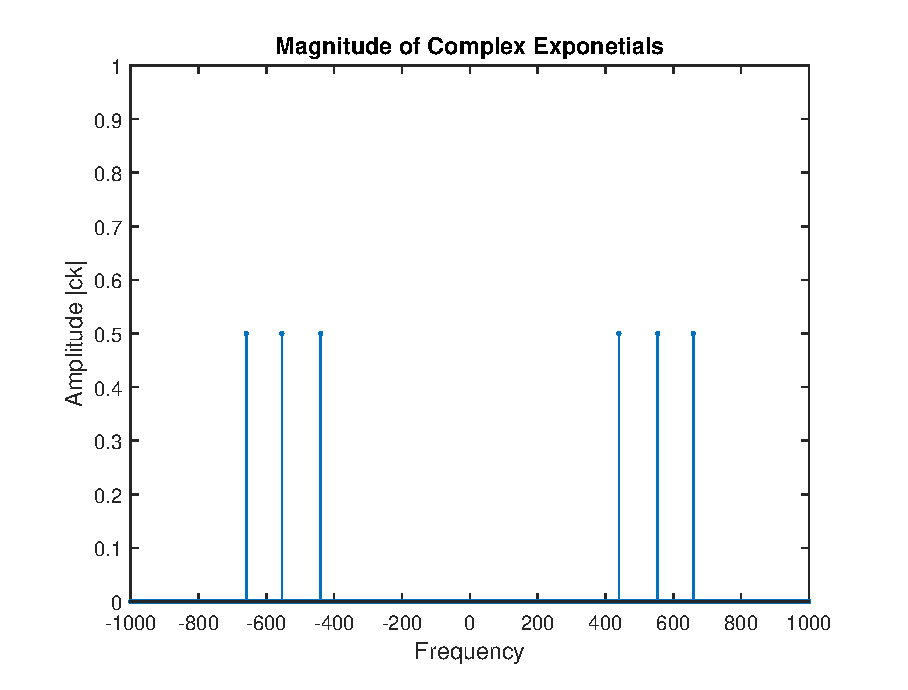
\includegraphics[scale=0.8]{fig1.eps}
    	\captionof{figure}{Magnitude of Complex Exponetials}
    \end{figure}
    
\end{homeworkProblem}



%%%%%%%%%%%%%%%%%%%%%%%%%%%%%%%%%%%%%%%%%%%%%%%%%%%%%%%%%%%%%%%%%%%%%%%%%%%%%%%%%%%%%%%%%%%%%%%%%%%%%%%%%%%%%%%%%%%%%%
% Question 4
%%%%%%%%%%%%%%%%%%%%%%%%%%%%%%%%%%%%%%%%%%%%%%%%%%%%%%%%%%%%%%%%%%%%%%%%%%%%%%%%%%%%%%%%%%%%%%%%%%%%%%%%%%%%%%%%%%%%%%

\begin{homeworkProblem}
    
    A Matlab function was written to apply an ideal low pass filter to the signal. The Matlab code can be seen below:
    
    \begin{lstlisting}
	    function ck_out = low_pass_filter(k,ck,w0,B)
	    
		    % Function has one output ck_out which is the output
		    % of the input signal with the filter applied to it.
		    % The inputs for the function are the fundamental
		    % frequency (w0), the input signal complex coefficients (ck),
		    % the bandwidth of the filter (B)
	    
		    filter = abs(-k:k) < (B/w0);
		    ck_out = ck.*filter;
		    
	    end
    \end{lstlisting}
    
    A Matlab script, implementing the above function, was written to plot the signal output for filters of bandwidth varying from 0 to 5000 $\si{\radian.\per\second}$. The script can be seen below:
    
    \begin{lstlisting}
	    % Script simply plots k vs ck for a signal composed of a finite number
	    % of cosine functions
	    
	    % Determine size of plot
	    n = 1000;
	    w0 = 2*pi;
	    
	    % Create values for k
	    k = -n:n;
	    
	    % Create storage vector for |ck|
	    pos_ck = zeros(1,n);
	    
	    % Insert ck amplitude into storage vector
	    A = [440 554 659];
	    pos_ck(A) = 0.5;
	    
	    % Compose |ck|
	    ck = [fliplr(pos_ck) 0 pos_ck];
	    ck_out = zeros(1,6);
	    
	    for i = 0:5
	    
		    % Run filter over input signal
		    ck_out = low_pass_filter(n,ck,w0,1000*i);
	    
		    % Create subplot template
		    subplot(3,2,i+1)
	    
		    % Plot individual stem plots for each B 
		    stem(k,ck_out,'marker','.')
		    title(sprintf('B: %d', 1000*i))
		    xlabel('Frequency')
		    ylabel('Amplitude |ck|')
		    axis([-1000 1000 0 1]);
		    
	    end
    \end{lstlisting}
    
    The plot can be seen in Figure 2.
    
    \begin{figure}[H]
    	\centering
    	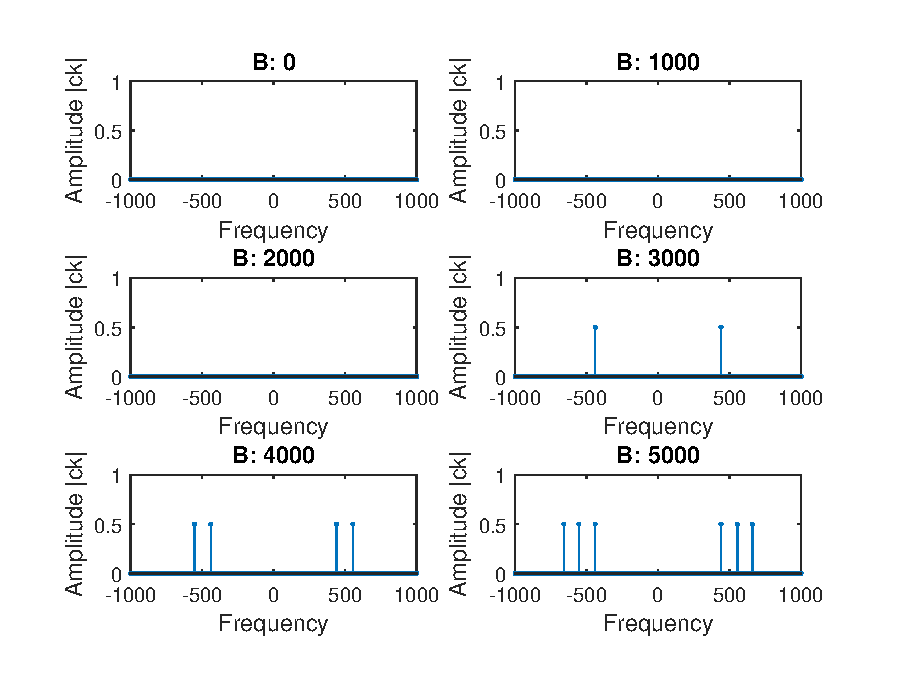
\includegraphics[scale=0.8]{fig2.eps}
    	\captionof{figure}{Magnitude of Complex Exponetials}
    \end{figure}
    
\end{homeworkProblem}

\newpage

%%%%%%%%%%%%%%%%%%%%%%%%%%%%%%%%%%%%%%%%%%%%%%%%%%%%%%%%%%%%%%%%%%%%%%%%%%%%%%%%%%%%%%%%%%%%%%%%%%%%%%%%%%%%%%%%%%%%%%
% Question 5
%%%%%%%%%%%%%%%%%%%%%%%%%%%%%%%%%%%%%%%%%%%%%%%%%%%%%%%%%%%%%%%%%%%%%%%%%%%%%%%%%%%%%%%%%%%%%%%%%%%%%%%%%%%%%%%%%%%%%%

\begin{homeworkProblem}
	
   Finally, the script from problem 4 was modified so that the filtered signal would play after each iteration of filtering. The code can be seen below:
   
   \begin{lstlisting}
	   % Script simply plots k vs ck for a signal composed of a finite number
	   % of cosine functions
	   
	   % Determine size of plot
	   n = 1000;
	   w0 = 2*pi;
	   
	   % Create values for k
	   k_pos = 1:n;
	   k = -n:n;
	   
	   % Create storage vector for |ck|
	   pos_ck = zeros(1,n);
	   
	   % Insert ck amplitude into storage vector
	   A = [440 554 659];
	   pos_ck(A) = 0.5;
	   
	   % Compose |ck|
	   ck = [fliplr(pos_ck) 0 pos_ck];
	   ck_out = zeros(1,6);
	   
	   % Set up sampling frequency and time duration to play back filtered signal
	   dur = 2.0;
	   fs = 44100;
	   t = 0:(1/fs):dur;
	   
	   for i = 0:5
	   
		   % Plot individual stem plots for each B
		   ck_out = low_pass_filter(n,ck,w0,1000*i);
		   subplot(3,2,i+1)
		   stem(k,ck_out,'marker','.')
		   title(sprintf('B: %d', 1000*i))
		   xlabel('Frequency')
		   ylabel('Amplitude |ck|')
		   axis([-1000 1000 0 1]);
		    
		   for j = 1:length(k_pos)
			   
			   % Check for magnitudes at frequency
			   if ck_out(j) ~= 0
				   
				   % Convert back to time series
				   x = ck_out(j)*( exp(1i*k(j)*w0*t) + exp(-1i*k(j)*w0*t) );
				   
				   % Exclude any complex exponentials
				   real_x = real(x);
				   sound(x,fs)
				   pause(3)
			   end
		   end
	   end
   \end{lstlisting}
    
\end{homeworkProblem}

\end{document}
